\section{Design}

This section of the document outlines all the key design decisions made when building WiredEmu, both internally and in terms of aesthetics and GUI design.

\subsection{Coding Style}
    Unlike perhaps most mainstream programming languages, C++ has no real consensus in terms of coding style, use of case and naming conventions. In order to maintain consistency across the project therefore, in this section I shall outline the code style adopted across the project (of course, external libraries often use various different styles that do not align with my own but that is unfortunately unavoidable).

    \subsubsection{Use of Case}
        Identifiers that should use camelCase:
        \begin{itemize}
            \item Local and member variables \texttt{int x;}
            \item Namespaces \texttt{namespace ns}
            \item Function and method names \texttt{void func()}
            \item Function and method parameters \texttt{void func(int parameter)}
        \end{itemize}

        Identifiers that should use PascalCase:
        \begin{itemize}
            \item Class names \texttt{class ClassName}
            \item Enumeration names \texttt{enum EnumName}
            \item Structure names \texttt{struct StructureName}
            \item Type definitions/aliases \texttt{using TypeName = ...;}
            \item Template parameters representing types \texttt{template <typename TypeTemplateParameter, unsigned int notTypeParameter>}
        \end{itemize}

        Identifiers that should use UPPER\_CASE:
        \begin{itemize}
            \item Macros \texttt{\#define MACRO\_NAME ...}
            \item Enumeration values \texttt{enum \{ FIRST\_VALUE, SECOND\_VALUE \};}
            \item Constants where the value is known at compile-time and will never change throughout the execution of the program (this is something which is not guaranteed when using the \texttt{const} keyword depending on how and where it is used)
        \end{itemize}

    \subsubsection{Whitespace}
        Spaces will be used instead of tab characters. A normal indentation should be four spaces. I chose to use spaces over regular tabs as they allow for one to be sure that more complex use of indentation will visually appear the same for all regardless of text editor used.

        All mathematical operators, with the exception of unary operators, should be padded with spaces on either side (for example, \texttt{10 + (2 * a)} and \texttt{-x + 5}).

        When using pointer or reference types, have the \texttt{*} or \texttt{\&} attached to the type name and not the identifier name (for example, \texttt{unsigned int* x;}).

        All elements in a single-line brace initialisation should be spaced as such (each element having a space on either side): \texttt{\{ 5, 10, 15 \}}

    \subsubsection{Naming Conventions}
        Names like \texttt{i} and \texttt{j} are acceptable for numerical counters for short loops. For longer loops or loops where a collection of items are iterated through then more descriptive names are preferred (for example, use \texttt{for(auto child : children)} instead of \texttt{for(auto i : children)}).

        Names for namespaces should be kept short whenever possible so as to discourage the use of \texttt{using namespace veryLongNamespaceName;} (names like \texttt{emu} or \texttt{gui} are acceptable for namespaces though make sure to document their purpose when using such short names).

        Class and type names are not recommended to be kept as short as namespace names and therefore can and should be more descriptive (for example, use \texttt{class InterruptHandler} instead of \texttt{class IntHandle}). Frequently used type aliases can have shorter names for the sake of convenience.

    \subsubsection{Examples}
        \begin{listing}[h]
            \inputminted{c++}{code/enum.cpp}
            \caption{Example of coding style to use when defining enumerations.}
            \label{lst:enum-example}
        \end{listing}

        \begin{listing}[h]
            \inputminted{c++}{code/class.hpp}
            \caption{Example of coding style to use when declaring a class or structure.}
            \label{lst:class-example}
        \end{listing}

\subsection{Project Structure}
    \label{sec:project-structure}
    As the most basic level, I opted for the typical C++ project structure wherein there are two primary directories: \texttt{src} (stores all source/implementation files) and \texttt{include} (stores all header files). It is standard practice when writing in C++ to keep the definition of classes, functions and data structures entirely separate from their implementation whenever possible as this allows for significantly improved build times when only minor changes to the code are made. Definitions are found in header files (\texttt{*.hpp}) in the \texttt{include} directory while implementations are found in source files (\texttt{*.cpp}) in the \texttt{src} directory. I considered using the new module system planned for C++ 20 over the header/source method, however support for modules is still somewhat patchy as the C++ 20 standard is not yet fully finalised at the time of writing.

    If in order to maintain a degree of modularity and allow for the use of the emulator core as a general-purpose library without any GUI/CLI/unit tests, I devised a system wherein the code base is split into four different groups/build targets: \texttt{common}, for all emulator and shared code; \texttt{cli}, for command-line interface code; \texttt{gui}, for graphical user interface code; and \texttt{test}, for unit testing. While \texttt{cli}, \texttt{gui} and \texttt{test} are executable build targets (i.e. they each have a \texttt{main} function and generate standalone executables), \texttt{common} is a non-executable library which is linked again each of the aforementioned executables.

    The directory structure inside of both \texttt{src} and \texttt{include} mirror the structure of the project's nested namespaces for the most part. For example, the definition of the class \texttt{emu::cpu::Intel8086} (part of the \texttt{common} build target) can be found in \texttt{include/common/emu/cpu/intel8086.hpp} and its implementation in \texttt{src/common/emu/cpu/intel8086.cpp}.

\subsection{Namespaces}
    \begin{itemize}
        \item \texttt{emu} - Contains all emulator code. Part of \texttt{common} build target.
        \begin{itemize}
            \item \texttt{emu::cpu} - Contains emulator code specific to the Intel 8086 Central Processing Unit.
            \begin{itemize}
                \item \texttt{emu::cpu::reg} - Code related to CPU registers.
                \item \texttt{emu::cpu::instr} - Code specific to the representation of CPU instructions.
            \end{itemize}
            %\item \texttt{emu::pic} - Contains code for the Intel 8259 Programmable Interrupt Controller.
            %\item \texttt{emu::pit} - Contains code for the Intel 8253 Programmable Interval Timer.
        \end{itemize}
        \item \texttt{convert} - Contains functions and function templates for the conversion between different types and formats of data. Part of \texttt{common} build target.
        \item \texttt{gui} - Contains all GUI code. Part of \texttt{gui} build target.
    \end{itemize}


\subsection{Build System}
    C++ is known for being notoriously complex and inconsistent to build across different platforms. Fortunately, tools like CMake make this \textit{somewhat} easier. CMake is a tool essentially for configuring whatever build system may be available on the given system. For example, on my Linux computer, CMake writes a Makefile which utilises the GCC compiler but, on Windows, it generates a Visual C++ Project file which uses Microsoft's Visual C++ compiler.

    CMake requires a configuration file called \texttt{CMakeLists.txt} which, despite having the \texttt{.txt} file extension, contains code in a domain-specific language unique to CMake. This allows one to specify the details of where header files are contained, which source files to compile, libraries to link against, and any other factors that may need to managed in order to build a codebase.

    My initial \texttt{CMakeLists.txt} was rather simple - it stated that the \texttt{include} directory contained header files, to recursively look in the \texttt{src} directory for source files, and that an executable called \texttt{WiredEmu} should be created.

    Naturally, as the project grew more complex, so did its build script. While initially the emulator had only a command-line interface, I soon decided it would be necessary to implement a full graphical user interface. In addition, it was believed that adding unit testing functionality would benefit the stability of the program and assist with debugging. The current build script and version of CMake used did not support such features. As such, I updated CMake and began to make use of its modern features - the primary of which being its build target system. It was this feature that allowed for the building of the various different executables described in section \ref{sec:project-structure}.

    Modern CMake allows the creation of distinct build targets which can each have unique properties for both themselves as well as for those they are linked against/depended on by. This is done by specifying public, private and interface properties with private properties applying only to the target; interface properties only applying to other targets dependent on the target; and public properties which are equivalent to applying both of the former. As an example, this would allow for a library to be built using C++ 17 (private property) but only require targets that depend on it to be built with a minimum of C++ 11 (interface property).


\subsection{GUI Design}
    \label{sec:gui-design}
    As you can see in the initial design in Figure \ref{figure:gui-first-design}, the GUI for this project was based primarily around three main components: a hex editor (shown in the top-left of the design), a status/control panel (bottom-left), and various register panels (right).

    \begin{figure}
        \centering
        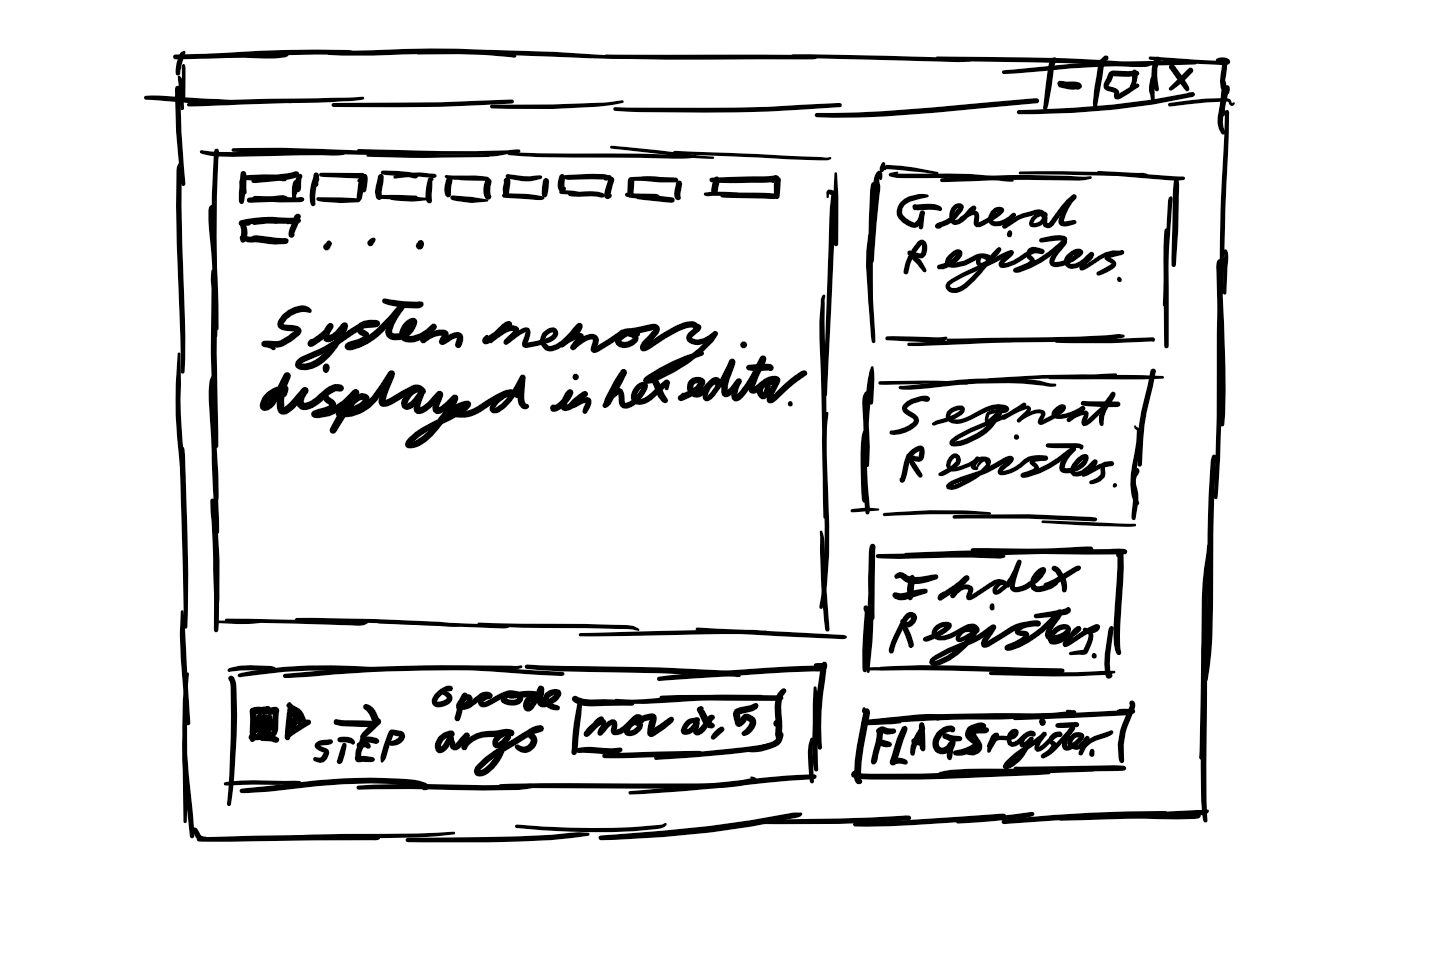
\includegraphics[scale=0.4]{gui-first-design}
        \caption{Initial GUI design drawn on a Surface Pro tablet.}
        \label{figure:gui-first-design}
    \end{figure}

    The hex editor would display and allow the user to alter system memory, the status/control panel would show the disassembled instruction currently being run and will the user to play/pause execution as well as change execution speed, while finally the register panels will each display and will allow for the editing of the values of all the different register groups (general-purpose, segments, index registers, stack registers and FLAGS register).

    A new design was created in order to be more applicable to use with the chosen GUI library (ImGui). See figure \ref{figure:gui-second-design}. This design differs from the previous one by having separate 'sub-windows' for the hex editor, control panel, and registers panels. In addition, this revised GUI design shows more of the specifics of the layout within even panel (the original design instead only showed the general arrangement of the panels themselves).

    \begin{figure}
        \centering
        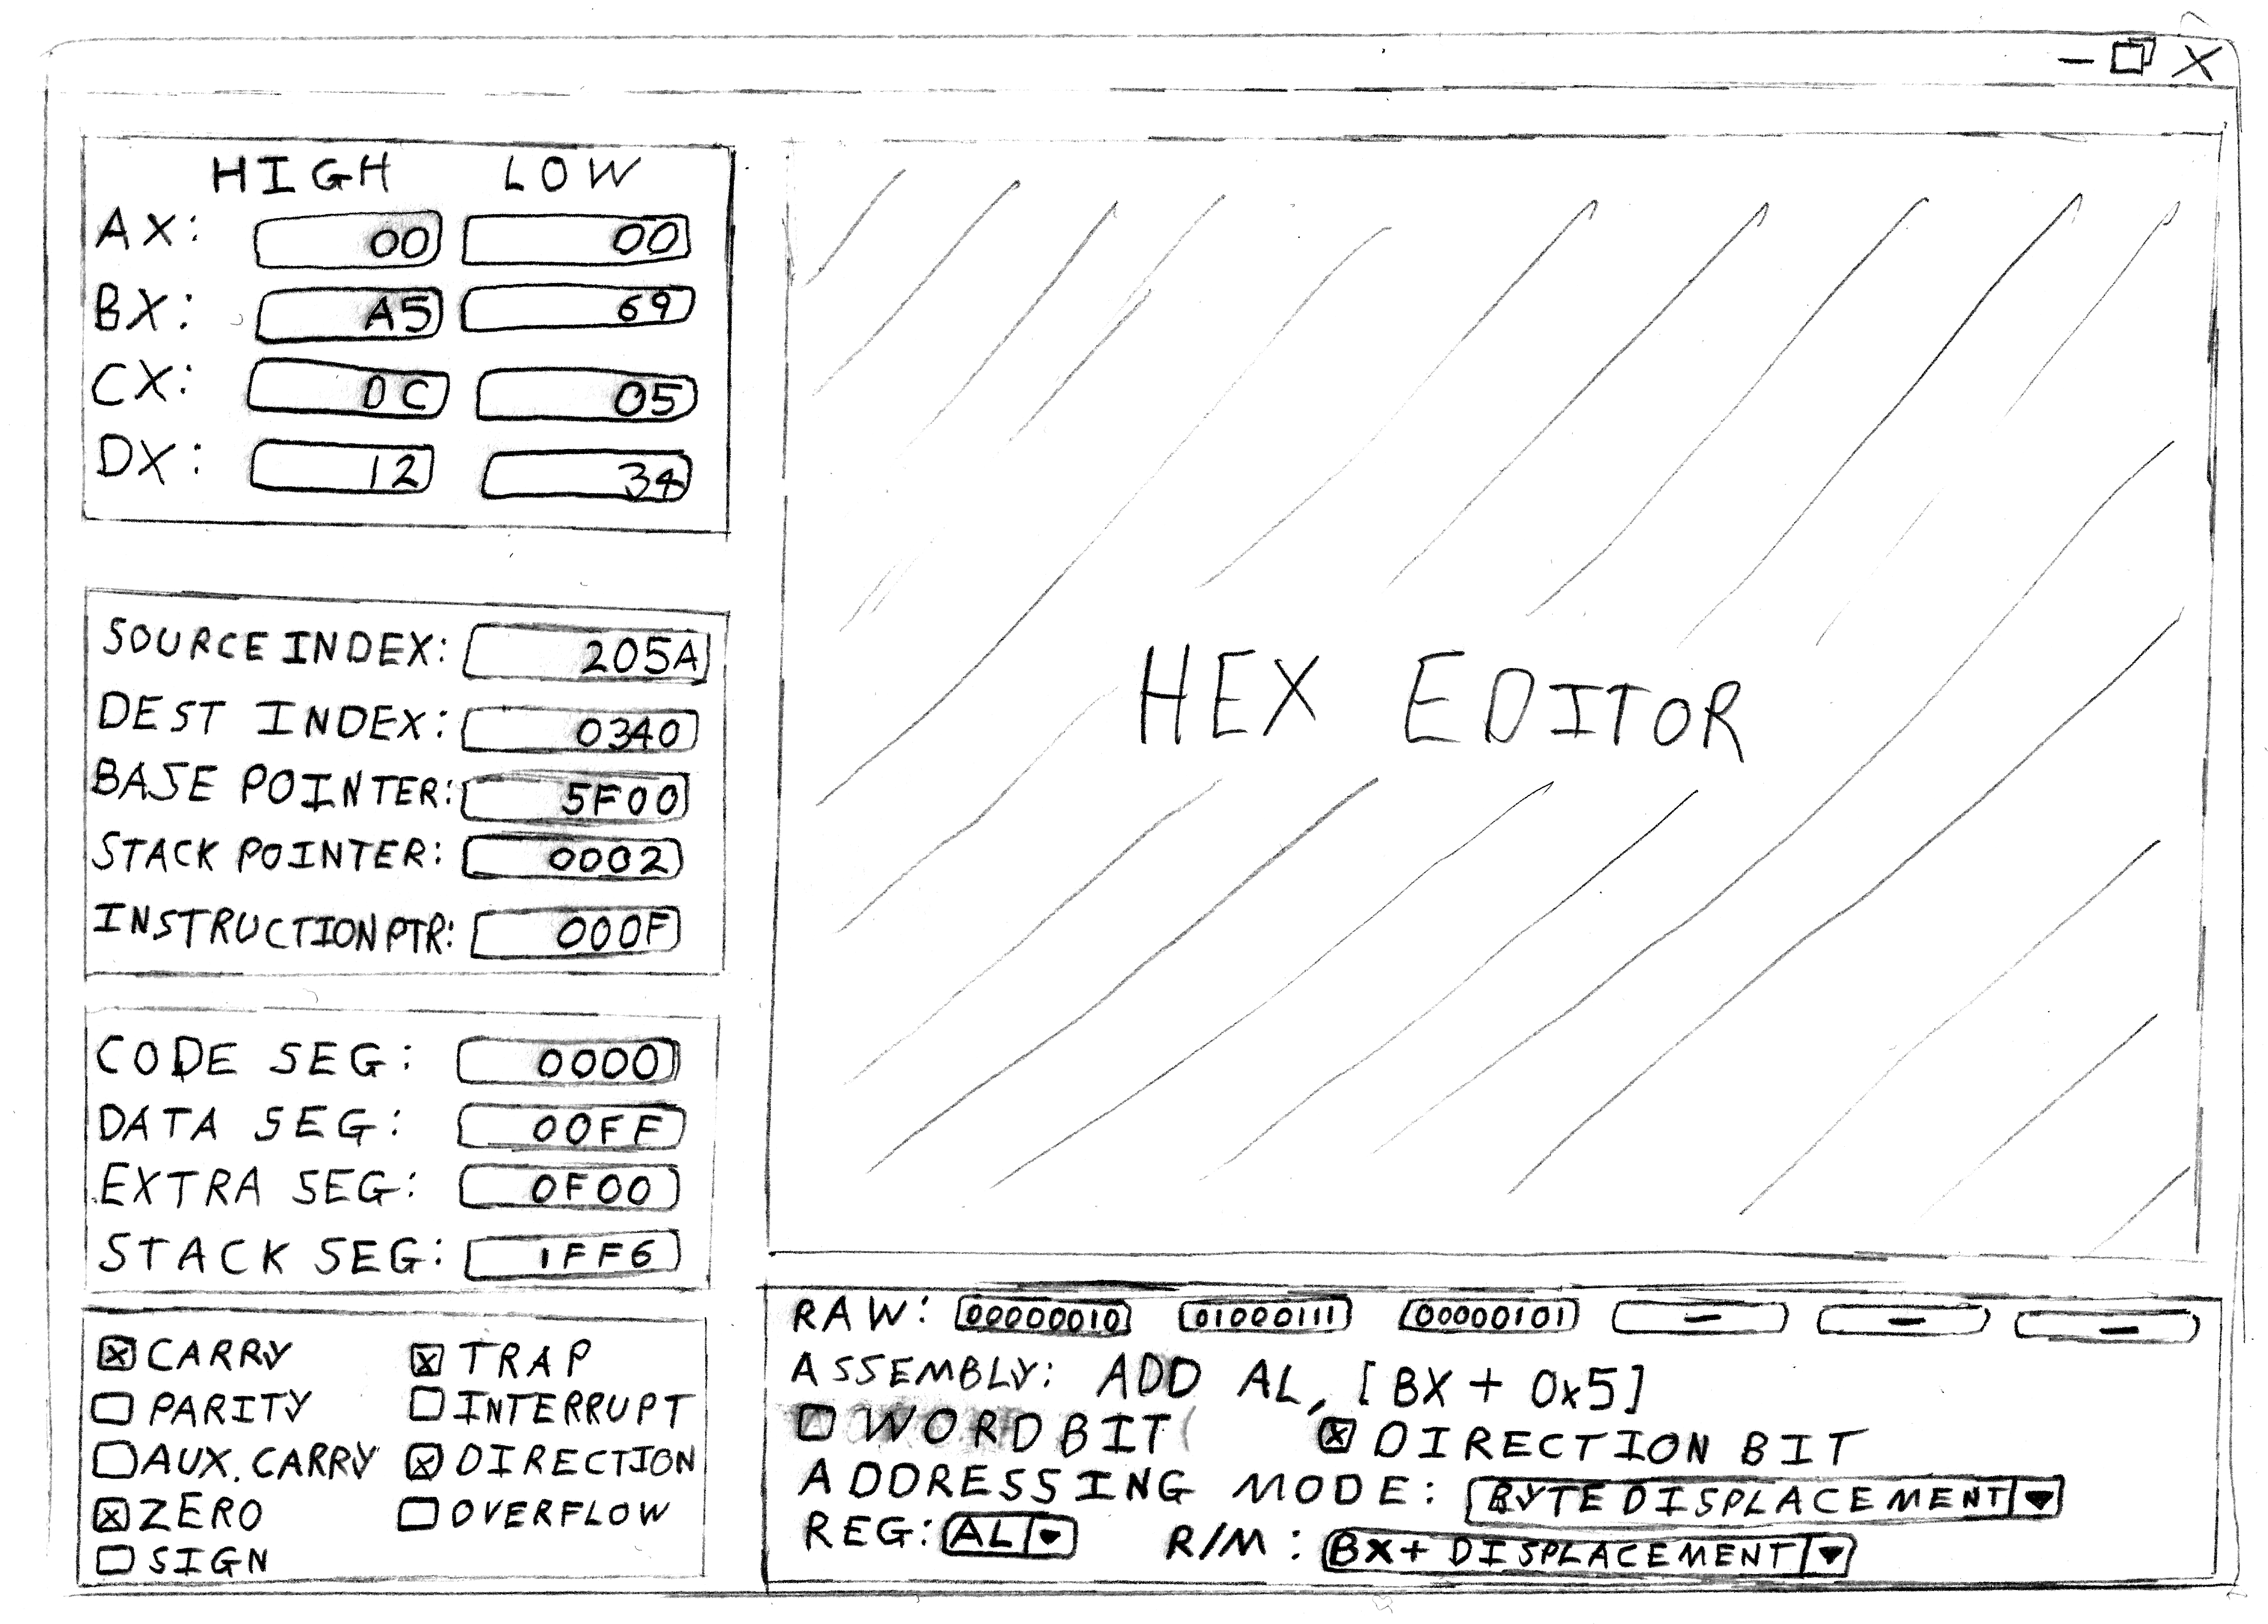
\includegraphics[scale=0.35]{gui-second-design}
        \caption{Revised GUI design drawn using pencil and paper.}
        \label{figure:gui-second-design}
    \end{figure}

    Down the left-hand side of this are collection of 4 register-related GUI panels. The first (top-left) shows the CPU's general-purpose 16-bit registers registers split into their two 8-bit components each (high and low bytes) in a 2 by 4 grid. This grid layout is ideal as it reduces the visual clutter of having three labelled fields each (AX, AH, AL, etc.) for what is effectively just a set of four single registers. Indeed, reducing the complexity of the GUI while still providing a high level of functionality is key, especially for the stakeholder's needs (use in a learning environment).

    Below the general-purpose registers panel are the index and segment register panels. Note how unlike many other emulators, my emulator will give the full name of each segment and index register rather than just the acronyms (for example, 'SOURCE INDEX' instead of just 'SI'). This felt necessary so that students did not have to constantly look up what each individual acronym means. In addition, since index and segment registers can only be accessed as full 16-bit values (not as individual high/low bytes like with the general-purpose registers), these panels do away with the 2 columns used in the general-registers panel.

    The bottom-left panel of the revised GUI design shows the CPU flags. While the nine status flags on the real Intel 8086 processor are stored as bits of a single 16-bit FLAGS register, my solution instead stores them as just a collection of nine boolean values. This GUI design follows suit by simply having each flag next to a checkbox toggle to clearly show whether it is or is not enabled. Full names of flags are also displayed instead of the shorthands/acronyms seen in many pieces of documentation (for example, 'PARITY' instead of 'PF').


\subsection{Instruction Representation}
    Decoded instructions are represented using complex data structures making heavy use of object-orientation and inheritance. This allows for logical encapsulation and for more efficient efficient code reuse. Note that the eplanations below do not provide full namespaces of the referenced objects/functions/etc so as to aid readability.

    The most basic instruction class is simply titled \texttt{Instruction} and holds basic attributes that are components of every x86 instruction. These include an opcode (represented using a \texttt{Opcode} object) and an assembly identifier (e.g. \texttt{add}, \texttt{jnz}). Note that this class is purely virtual/abstract and cannot be initiated without the overriding of its three virtual methods.

    One method of \texttt{Instruction} that should be  overridden is: \mint[linenos=false]{c++}{virtual OffsetAddr execute(Intel8086& cpu, Mem& memory) = 0;}

    As the name would suggest, it is the role of this method to executed the instruction using the given \texttt{cpu} and \texttt{memory} references. Note that these are mutable (i.e. non-constant) references meaning modification is allowed (an instruction unable to modify CPU or memory state would naturally have very limited use). This is in contrast to the \texttt{toAssembly} method discussed shortly which takes constant references so as to prevent accidental modification of the passed CPU and memory.

    The \texttt{execute} method is required to return an \texttt{OffsetAddr} (an alias for a unsigned 16-bit integer type). The CPU's instruction pointer will be set to this returned value on execution completion. For most instructions other than jump and interrupt instructions, the address of the next instruction (and thus the appropriate return value) will simply by the current instruction pointer plus the length of the encoded instruction in bytes. As such, a helper method is provided: \mint[linenos=false]{c++}{OffsetAddr nextAddress(const Intel8086& cpu) const;}
    
    The above helper method allows most instructions to end their \texttt{execute} method simply with the statement: \mint[linenos=false]{c++}{return nextAddress(cpu);}

    The \texttt{Instruction} class also has the following virtual method: \mint[linenos=false]{c++}{virtual std::string toAssembly(const Intel8086& cpu, const assembly::Style& style) const;}

\subsection{Usability Features}
    For a piece of software that is supposed to be used by students not yet acutely familiar with processor architecture, the usability of said software is a key concern.

    The first major consideration when it comes to usability, is the general layout of the software's GUI. One issue with many similar solutions is an intimidating and complex-to-navigate user interface. This is something I hope to address properly with my own solution. Please see section \ref{sec:gui-design} for a breakdown for the GUI design process and an outline of some more general usability features of the software.

    After discussions with the shareholder, we agreed on a particular feature designed to aid usability of the software to quite an extent. This feature is the introduction of 'tool tips' - short paragraphs of description displayed when the user hovers their mouse over a particular area of the GUI. This is beneficial as it allows for details on appropriate software usage to be provided in a streamlined manner (e.g. without having to refer to separate usage instructions). In addition, having this information only appear on mouse hover prevents additional clutter in what is already a somewhat intimidating user interface.

\subsection{Testing}
    Naturally, it is difficult to decide on the specifics of testing before any code has actually been written. The current plan is to write a collection of unit tests during the iterative development process in order to test the internals of the software.

    \subsubsection{Unit Testing}
        When working on larger projects with expansive code bases, it can quickly become inconvenient to manually test each individual portion of said code base. Fortunately, unit testing allows for a degree of automation in the process of ensuring each component or 'unit' that makes up a piece of software functions as it should. This is typically done by writing tests that give certain inputs to pieces of code and will only pass should the expected outputs are received. Should a test fail then a report explaining which portion of code failed, what it was supposed to do, and what it actually did is generated.

        Initially I wrote my own unit testing framework. This framework was built around constructing an object holding a 'test function' (lambda/anonymous function) which performs an assertion by either returning true to indicate a pass and false to indicate failure. This unit test object then had various methods available which allowed one to pass input to the testing function and then have the result of its assertion handled appropriately.

        While this method did indeed work, it presented a couple of issues. The first of which being the limited information given when a test failed. I had made a \texttt{CREATE\_TEST} macro which passed information such as in which file and function the test was created to the the unit test object, which gave some degree of insight into how to test failed. More information such as the precise value of arguments to the test function however, would be helpful to provide for debugging purposes. While I was able to just use parameter pack expansion in order the write most argument values to standard output, more complex values (such as \texttt{std::vector} values or values of custom types) cannot be handled be \texttt{std::cout} by default. While I could have written a custom output stream derived from \texttt{std::ostream} to handle these types, doing so would be rather time consuming.

        Another issue with my own unit testing framework was the lack of categorisation of tests. The implementation did not allow for the tagging or running of individual tests and instead always ran every test defined. This was inefficient and did not allow for optimal organisation when a large quantity of tests are defined.

        After realising that improving my own unit testing framework could be an entire project in and of its self, I decided to utilise a third-party framework so that I would be able to place all focus on coding the emulator portion of the project. The framework I chose after a few days of deliberation was \textbf{Catch2}. Features that drew me to this particular framework include the ability to search for and tag tests, the fact that far more detailed information about failed tests are provided, and the ability provided by this framework to split tests into separate subsections.
    \subsubsection{Assembly Generation}
        Every CPU cycle, the instruction at the point in memory indicated by the instruction pointer is converted into its human-readable assembly representation. This assembly representation is displayed to the user so that it is clear to them what an instruction will do before it is actually run. I concluded the best way to test the validity of the emulator's generated assembly would be compare it to that of a pre-existing disassembler.

        The GNU project provides a piece of software \texttt{objdump} which allows for the in-depth analysis of object code. Using the command-line \texttt{-D} option, \texttt{objdump} will produce assembly code from the specified object file. The \texttt{-Mintel} option is employed also so as to specify the use Intel x86 syntax rather than AT\&T as the former is the style I have programmed the emulator to output. The argument \texttt{-m i8086} is used to specify the Intel 8086 as the target architecture. For the sake of completeness, the \texttt{-b binary} option is also used to specify the input file's binary format (including this option is not really necessary as \texttt{objdump} is quite good at inferring the format used).

        Disassembling the code in a file called \texttt{a.out} could therefore be done with the following command: \mint[linenos=false]{bash}{objdump -Mintel -D -b binary -m i8086 a.out}

        I would perform these tests based on each general type of instruction so as to ensure each variety is functional.

    \subsubsection{Instruction Execution}
        Ensuring instructions actually perform the correct changes to CPU state (i.e. execute correctly) is to be done using a collection of unit tests. As mentioned in the Analysis section, I will use the Catch2 library for creating, managing, and running unit tests.

        \inputminted{c++}{code/testexample.cpp}

        Above is an example of what one such unit test may look like. This approach is ideal as it allows me to test all instructions by simply running the generated unit testing executable.

    \subsubsection{Emulator Memory}
        Having memory representation for the emulated system that functions as expected is also vital as any system, emulated or otherwise, will frequently write to and read from memory. Again, unit testing is ideal in this situation.

        Testing data table \ref{table:memory-test-data} works on the assumption that memory consists of a total of 0xFF separate 8-bit values.

        \begin{table}
            \begin{tabular}{ | c | c | m{0.3\textwidth} | }
                \hline
                Test Data & Type & Description \\
                \hline
                write byte to address \texttt{0x0F} & normal & write byte value to valid memory address (within bounds) \\
                write byte to address \texttt{0xFE} & boundary & write byte value to address just within memory bounds \\
                write byte to address \texttt{0x5FF} & erroneous & attempt to write memory value that is out-of-bounds so exception should be thrown \\
                write several bytes beginning from address \texttt{0x10} & normal & to valid memory addresses (within bounds) \\
                write several bytes beginning from address \texttt{0xFD} & erroneous & not all memory addresses will be within bounds so exception should be thrown \\
                read byte from address \texttt{0x0F} & normal & read byte from valid memory address (within bounds) \\
                read byte from address \texttt{0xFE} & boundary & read byte from address just within memory bounds \\
                read byte from address \texttt{0xABCD} & erroneous & attempt to read byte that is out-of-bounds so exception should be thrown \\
                read several bytes from address \texttt{0x15} & normal & from valid memory addresses (within bounds) \\
                read several bytes from address \texttt{0xFD} & erroneous & not all memory addresses will be within bounds so exception should be thrown \\
                \hline
            \end{tabular}
            \caption{Table of emulator memory test data.}
            \label{table:memory-test-data}
        \end{table}

    \subsubsection{Memory Segmentation}
        As before, unit testing will also be used for the testing of memory segmentation. See table \ref{table:segmentation-test-data}.

        \begin{table}
            \begin{tabular}{ | c | c | c | c | }
                \hline
                Segment Register Value & Offset Value & Expected Absolute Address & Test Data Type \\
                \hline
                \texttt{0000} & \texttt{0000} & \texttt{00000} & normal \\
                \texttt{00FF} & \texttt{0000} & \texttt{000FF} & normal \\
                \texttt{00FF} & \texttt{000F} & \texttt{00FFF} & normal \\
                \texttt{FFFF} & \texttt{000E} & \texttt{FFFFE} & boundary \\
                \texttt{FFFF} & \texttt{FFFF} & - & erroneous \\
                \hline
            \end{tabular}
            \caption{Table of memory segmentation testing data.}
            \label{table:segmentation-test-data}
        \end{table}

    \subsubsection{Post-Development Testing}
        ...
